\RequirePackage{luatex85}
\documentclass[tikz]{standalone}
% Default preamble
\usepackage{pgfplots}
\pgfplotsset{compat=newest}

\begin{document}
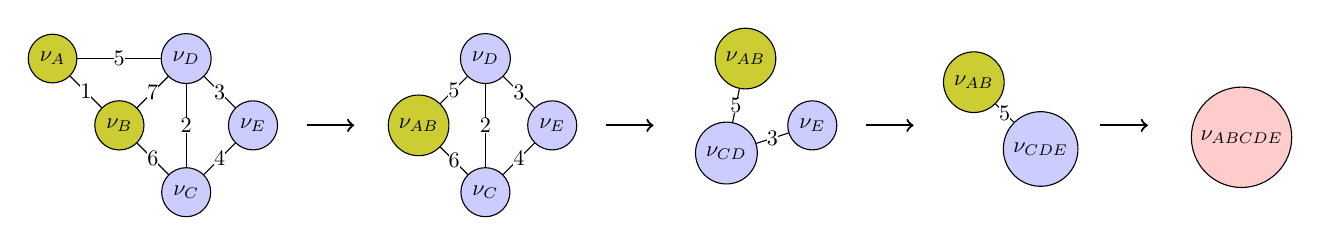
\begin{tikzpicture}[scale=1, every node/.style={scale=0.8}]
\tikzset{classA/.style={circle, draw=black, fill=blue!20!yellow}, node distance=1.5cm}
\tikzset{classB/.style={circle, draw=black, fill=blue!20}, node distance=1.5cm}
\tikzset{classX/.style={circle, draw=black, fill=red!20}, node distance=1.5cm}
  \begin{scope}
    \node[classA] (A) {$\nu_{A}$};
    \node[classA, below right of=A] (B) {$\nu_{B}$};
    \node[classB, below right of=B] (C) {$\nu_{C}$};
    \node[classB, above right of=B] (D) {$\nu_{D}$};
    \node[classB, below right of=D] (E) {$\nu_{E}$};
    \draw [-] (A) -- (B) node [midway, fill=white, inner sep=0px] {1};
    \draw [-] (A) -- (D) node [midway, fill=white, inner sep=0px] {5};
    \draw [-] (C) -- (D) node [midway, fill=white, inner sep=0px] {2};
    \draw [-] (D) -- (E) node [midway, fill=white, inner sep=0px] {3}; 
    \draw [-] (C) -- (E) node [midway, fill=white, inner sep=0px] {4};  
    \draw [-] (C) -- (B) node [midway, fill=white, inner sep=0px] {6};    
    \draw [-] (D) -- (B) node [midway, fill=white, inner sep=0px] {7};
    \draw[->, thick] ([xshift=4.5ex] E.center) -- ([xshift=8.5ex] E.center);
  \end{scope}
  
  \begin{scope}
  [xshift=3.8cm]
    \node (A) {};
    \node[classA , below right of=A] (AB) {$\nu_{AB}$};
    \node[classB, below right of=AB] (C) {$\nu_{C}$};
    \node[classB, above right of=AB] (D) {$\nu_{D}$};
    \node[classB, below right of=D] (E) {$\nu_{E}$};
    \draw [-] (AB) -- (D) node [midway, fill=white, inner sep=0px] {5};
    \draw [-] (C) -- (D) node [midway, fill=white, inner sep=0px] {2};
    \draw [-] (D) -- (E) node [midway, fill=white, inner sep=0px] {3}; 
    \draw [-] (C) -- (E) node [midway, fill=white, inner sep=0px] {4};  
    \draw [-] (C) -- (AB) node [midway, fill=white, inner sep=0px] {6}; 
    \draw[->, thick] ([xshift=4.5ex] E.center) -- ([xshift=8.5ex] E.center);
  \end{scope}  
  
  \begin{scope}
  [xshift=8.8cm]
    \node[classA] (AB) {$\nu_{AB}$};
    \node[classB, below of=AB, xshift=-2ex] (CD) {$\nu_{CD}$};
    \node[classB, below right of=AB] (E) {$\nu_{E}$};
    \draw [-] (AB) -- (CD) node [midway, fill=white, inner sep=0px] {5};
    \draw [-] (CD) -- (E) node [midway, fill=white, inner sep=0px] {3}; 
    \draw[->, thick] ([xshift=4.5ex] E.center) -- ([xshift=8.5ex] E.center);
  \end{scope} 
  
  \begin{scope}
  [xshift=11.7cm, yshift=-0.3cm]
    \node[classA] (AB) {$\nu_{AB}$};
    \node[classB, below right of=AB] (CDE) {$\nu_{CDE}$};
    \draw [-] (AB) -- (CDE) node [midway, fill=white, inner sep=0px] {5};
    \draw[->, thick] ([xshift=5ex, yshift=0.3cm] CDE.center) -- ([xshift=9ex, yshift=0.3cm] CDE.center);    
  \end{scope}    
  
   \begin{scope}
  [xshift=15.1cm, yshift=-1cm]
    \node[classX] (ABCDE) {$\nu_{ABCDE}$};
  \end{scope}
\end{tikzpicture}
\end{document}
